\documentclass{article}

\usepackage[utf8]{inputenc}
\usepackage[T1]{fontenc}
\usepackage[french]{babel}
\usepackage{fancyhdr}
\usepackage{listings}
\usepackage{graphicx}

\pagestyle{fancy}
\lstset{language=bash}
\rhead[]{Projet de C++ : Sokochez}
\lhead[Projet de C++ : Sokochez]{}
\begin{document}
\title{Projet de C++ : Sokochez}
\date{}
\maketitle

\section{Introduction}

Dans le cadre de ce projet, nous avons réalisé une version multijoueur du jeu Sokoban qui consiste à ranger des caisses en les poussant. \\

\section{Fonctionnalités}

Les fonctionnalités que nous avons ajoutées sont les suivantes :
\begin{itemize}
    \item Affichage de couleurs dépendant du type d'objet
    \item Chargement du ou des niveaux depuis un ou plusieurs fichiers texte passés en argument
    \item Détection du mode de jeu en fonction de la carte chargée
    \item Affichage des règles en fonction du mode de jeu
    \item Affichage du nom du niveau
    \item Détection des niveaux erronés
    \item Trois modes de jeu :
    \begin{enumerate}
        \item Les joueurs doivent se rencontrer
        \item Les blocs A et B doivent être mis côte à côte
        \item Le bloc A doit être mis à coté de la position a, le B à coté de b…
    \end{enumerate}
    \item Un menu permettant de :
    \begin{enumerate}
        \item Passer au niveau suivant
        \item Recommencer le niveau
        \item Quitter le jeu
    \end{enumerate}
    \item Mode non-canonique
    \item Affichage de la solution utilisée en fin de niveau sous forme de chaîne de caractères
    \item Affichage du nombre de coups effectués pour réussir le niveau.
    \item Éditeur de niveaux comprenant :
    \begin{enumerate}
        \item Une jolie barre d'objets à placer
        \item Une touche d'optimisation du niveau enlevant les bordures inutiles
        \item Une touche de sauvegarde
    \end{enumerate}
\end{itemize}

\section{Comment jouer}

Les niveaux sont de simples fichiers texte. 
Pour charger un niveau, il faut le passer en argument au lancement du programme.
\begin{lstlisting}
./jeu niveau.txt
\end{lstlisting}
Plusieurs niveaux peuvent être passés en arguments, ils seront lancés à la suite.
\begin{lstlisting}
./jeu niveaux/*
./jeu niveau1.txt niveau2.txt
\end{lstlisting}
Il faut ensuite lire les règles qui sont affichées au chargement du niveau.
Les touches de déplacement sont \emph{zqsd} pour le joueur 1 et \emph{oklm} pour le joueur 2.
La touche de menu est \emph{v}.

\section{Éditeur de niveaux}
Pour lancer l'éditeur de niveaux, le premier argument passé au programme doit être \emph{-e}.
\begin{lstlisting}
./jeu -e niveau1.txt
./jeu -e niveau1.txt niveau2.txt
\end{lstlisting}
Cet éditeur permet de créer et modifier des niveaux adaptés au jeu.

\begin{center}
    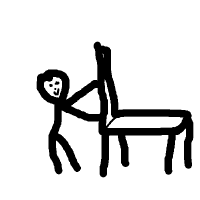
\includegraphics[width=200px,height=200px]{logo.png}
\end{center}

\end{document}
